\documentclass[9pt,aspectratio=169,xcolor=table]{beamer}

%~~~~~~~~~~~~~~~~~~~~~~~~~~~~~~~~~~~~~~~~~~~~~~~~~~~~~~~~~~~~~~~~~~~~~~~~~~~~~~
% Use roboto Font (recommended)
\usepackage[sfdefault]{roboto}
\usepackage[utf8]{inputenc}
\usepackage[T1]{fontenc}
%~~~~~~~~~~~~~~~~~~~~~~~~~~~~~~~~~~~~~~~~~~~~~~~~~~~~~~~~~~~~~~~~~~~~~~~~~~~~~~

%~~~~~~~~~~~~~~~~~~~~~~~~~~~~~~~~~~~~~~~~~~~~~~~~~~~~~~~~~~~~~~~~~~~~~~~~~~~~~~
% Define where theme files are located. ('/styles')
\usepackage{styles/fluxmacros}
\usefolder{styles}
% Use Flux theme v0.1 beta
% Available style: asphalt, blue, red, green, gray
\usetheme[style=hunter]{flux}
%~~~~~~~~~~~~~~~~~~~~~~~~~~~~~~~~~~~~~~~~~~~~~~~~~~~~~~~~~~~~~~~~~~~~~~~~~~~~~~

%~~~~~~~~~~~~~~~~~~~~~~~~~~~~~~~~~~~~~~~~~~~~~~~~~~~~~~~~~~~~~~~~~~~~~~~~~~~~~~
% Extra packages
\usepackage{booktabs}
\usepackage{colortbl}
\usepackage{ragged2e}
\usepackage{amssymb}
\usepackage{multirow}
\usepackage{tikz}
\usetikzlibrary{arrows.meta, positioning, fit, backgrounds, calc, decorations.pathreplacing}
\setbeamertemplate{itemize items}[square]
\usepackage[scaled=.8]{beramono}
\usepackage{listings}
\usepackage{styles/lstlangarm}
\usepackage{array}
\definecolor{bgcolor}{HTML}{F2E9E9}
% lstlangarm.sty references \color{mauve} for string literals but never defines
% it -- only fires when a listing contains a string. Define it here.
\definecolor{mauve}{rgb}{0.58,0,0.82}
% lstlangarm's C style sets commentstyle=green!20, which is unreadable on the
% pink listing background. Darken it globally.
\lstset{commentstyle=\color{green!45!black}}
% ragged-right fixed-width column -- must be defined in the preamble, never
% inside a frame (\newcolumntype's #1 breaks beamer's frame scanner)
\newcolumntype{R}[1]{>{\RaggedRight\arraybackslash}p{#1}}
%~~~~~~~~~~~~~~~~~~~~~~~~~~~~~~~~~~~~~~~~~~~~~~~~~~~~~~~~~~~~~~~~~~~~~~~~~~~~~~
% Table striping: odd rows white, even rows very light gray.
% Needs \documentclass[...,xcolor=table]{beamer} (beamer loads xcolor itself,
% so the option must go on the class, not \usepackage).
\definecolor{stripe}{gray}{0.94}
% \striped makes body rows alternate white, gray, white, ... starting white.
% \rowcolors counts from the first coloured body row; the header is not counted.
\newcommand{\striped}{\rowcolors{1}{white}{stripe}}
%~~~~~~~~~~~~~~~~~~~~~~~~~~~~~~~~~~~~~~~~~~~~~~~~~~~~~~~~~~~~~~~~~~~~~~~~~~~~~~

%~~~~~~~~~~~~~~~~~~~~~~~~~~~~~~~~~~~~~~~~~~~~~~~~~~~~~~~~~~~~~~~~~~~~~~~~~~~~~~
% TikZ block styles -- matches ch1/ch2
% Colour variables are named identically in the book's stm32primer.tex, so any
% tikzpicture using only the \tikzset{...} styles below can be copied verbatim
% between slides and book. Only the \definecolor/\colorlet VALUES differ: the
% book is printed, so it keeps every stroke pure black with muted fills. These
% slides are projected, so both fill AND stroke are bright and saturated to
% grab attention -- see stm32primer.tex for the print palette.
\definecolor{blkfill}{HTML}{DDEEDD}
\definecolor{blkline}{HTML}{355E3B}
\definecolor{accentfill}{HTML}{FFE0B2}
\definecolor{accentline}{HTML}{E65100}
\definecolor{memfill}{HTML}{DFF5DA}
\definecolor{memline}{HTML}{2E7D32}
\definecolor{cellfill}{HTML}{FFFFFF}
\definecolor{cellline}{HTML}{424242}
\definecolor{bitmaskfill}{HTML}{DCEBFF}
\definecolor{bitmaskline}{HTML}{1565C0}
\definecolor{bithitfill}{HTML}{FFE0B2}
\definecolor{bithitline}{HTML}{E65100}
\tikzset{
  blk/.style   = {rectangle, rounded corners=2pt, draw=blkline, fill=blkfill,
                  thick, align=center, font=\small, minimum height=9mm, inner sep=3pt},
  cpublk/.style= {rectangle, rounded corners=2pt, draw=accentline, fill=accentfill,
                  thick, align=center, font=\small\bfseries, minimum height=9mm, inner sep=3pt},
  memblk/.style= {rectangle, rounded corners=2pt, draw=memline, fill=memfill,
                  thick, align=center, font=\small, minimum height=9mm, inner sep=3pt},
  cell/.style  = {rectangle, draw=cellline, fill=cellfill, align=center,
                  font=\small\ttfamily, minimum height=7mm, inner sep=2pt},
  bitcell/.style={rectangle, draw=cellline, fill=cellfill, thick,
                  minimum width=5.4mm, minimum height=5.4mm, inner sep=0pt,
                  font=\scriptsize\ttfamily, anchor=center},
  bitmask/.style={bitcell, fill=bitmaskfill, draw=bitmaskline},
  bithit/.style ={bitcell, fill=bithitfill, draw=bithitline, font=\scriptsize\ttfamily\bfseries},
  rowlab/.style ={font=\scriptsize, text=Gray, anchor=east},
  oplab/.style  ={font=\scriptsize\itshape, text=Gray, anchor=west},
  lbl/.style   = {font=\scriptsize, text=Gray},
  flow/.style  = {-{Stealth[length=2mm]}, thick, draw=blkline},
  busline/.style={thick, draw=cellline},
}
% NOTE (theme quirks -- all fail SILENTLY, always page through the PDF):
%  - a second \\ inside a nested {...} group in a TikZ node breaks parsing
%  - {\small ...} wrapped around a nested itemize eats the frame title + list
%  - \usebeamercolor on a [plain] frame falls through to an unstyled default
%  - \newcolumntype inside a frame breaks beamer's frame scanner
%  - lstlisting needs \begin{frame}[fragile]
%  - a TikZ picture wider than its column silently overflows into neighbours
%~~~~~~~~~~~~~~~~~~~~~~~~~~~~~~~~~~~~~~~~~~~~~~~~~~~~~~~~~~~~~~~~~~~~~~~~~~~~~~

%%%%%%%%%%%%%%%%%%%%%%%%%%%%%%%%%%%
%% BEGIN CONDITIONAL COMPILATION %%
%%%%%%%%%%%%%%%%%%%%%%%%%%%%%%%%%%%
\newif\ifwebex
%\webextrue % uncomment to generate section separator
\ifwebex
\AtBeginSection[]{
  \begin{frame}
  \vfill
  \centering
  \begin{beamercolorbox}[sep=8pt,center,shadow=true,rounded=true]{title}
    \usebeamerfont{title}\insertsectionhead\par%
  \end{beamercolorbox}
  \vfill
  \end{frame}
}
\else
\AtBeginSection[]
{
{
    \setbeamercolor{background canvas}{bg=yellow!10}
    \begin{frame}[plain]
        \frametitle{Table of Contents}
        \tableofcontents[currentsection]
    \end{frame}
}
}
\fi
%%%%%%%%%%%%%%%%%%%%%%%%%%%%%%%%%%%
%% END CONDITIONAL COMPILATION   %%
%%%%%%%%%%%%%%%%%%%%%%%%%%%%%%%%%%%

%~~~~~~~~~~~~~~~~~~~~~~~~~~~~~~~~~~~~~~~~~~~~~~~~~~~~~~~~~~~~~~~~~~~~~~~~~~~~~~
% Information
\title{Introduction}
\subtitle{\emph{Contemporary Digital Electronic Systems} --- Chapter 1}
\author{Mun\'{i}m Zabidi}
\institute{\color{primary}Faculty of Electrical Engineering, Universiti Teknologi Malaysia}
\date{\today}
\titlegraphic{assets/logoutmwhite.png}
\graphicspath{{.}{../fig/}}
%~~~~~~~~~~~~~~~~~~~~~~~~~~~~~~~~~~~~~~~~~~~~~~~~~~~~~~~~~~~~~~~~~~~~~~~~~~~~~~

\begin{document}

\titlepage

%===============================================================================
\section{Why This Chapter}
%===============================================================================

\begin{frame}{Why This Chapter Matters}
  \begin{columns}[c]
  \begin{column}{.47\textwidth}
    Your phone, the car it rode in, the appliance it is charging on: each has a \alert{digital electronic system} at its core. This chapter sets up the vocabulary and mental model for the rest of the module.
  \end{column}
  \begin{column}{.51\textwidth}
    \begin{block}{After this chapter, you can:}
    {\small
    \begin{enumerate}\itemsep2pt
      \item Distinguish analog from digital quantities.
      \item Describe the voltage-range abstraction behind logic values.
      \item Qualify claims such as ``repeatable'' and ``noise-tolerant''.
      \item Name the digital IC types---ASIC, FPGA, CPLD, MCU, MPU, SoC.
      \item Read a timing diagram.
    \end{enumerate}}
    \end{block}
  \end{column}
  \end{columns}
\end{frame}

\begin{frame}{An Opening Question}
  \leavevmode\vspace{4mm}
  A thermometer, a speedometer and a stopwatch all measure things.
  \vspace{4mm}
  \begin{center}
  \fbox{\parbox{.78\textwidth}{\centering\vspace{2mm}
  \large Which should use a \alert{digital} representation internally, and which an \alert{analog} one?
  \vspace{2mm}}}
  \end{center}
  \vspace{4mm}
  By the end of this chapter you should be able to defend an answer.
\end{frame}

%===============================================================================
\section{Analog and Digital Quantities}
%===============================================================================

\begin{frame}{Analog versus Digital}
  \begin{columns}[c]
  \begin{column}{.5\textwidth}
    \centering
    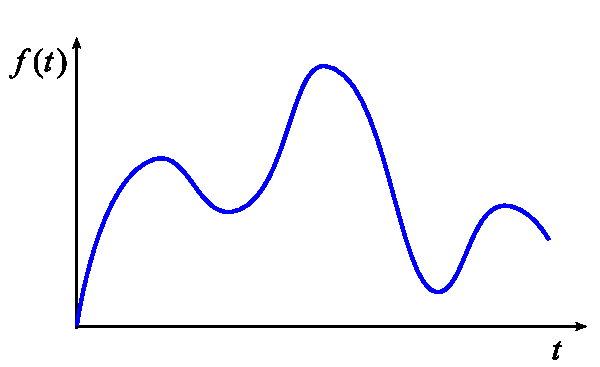
\includegraphics[width=\textwidth]{signal-analog}\\
    {\small Analog: any value in a range}
  \end{column}
  \begin{column}{.5\textwidth}
    \centering
    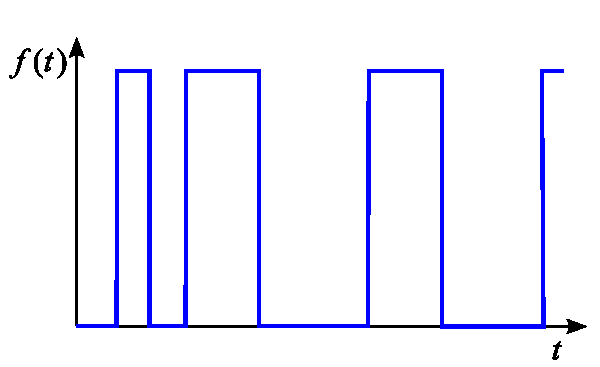
\includegraphics[width=\textwidth]{signal-digital}\\
    {\small Digital: a few discrete values}
  \end{column}
  \end{columns}
  \vspace{3mm}
  \begin{itemize}
    \item Digital circuits use only \alert{two} logic values: TRUE/FALSE, ON/OFF, HIGH/LOW.
    \item We therefore use binary numbers; each digit is a \alert{bit} (\textit{bi}nary digi\textit{t}).
  \end{itemize}
\end{frame}

\begin{frame}{Why Digital?}
  \begin{columns}[t]
  \begin{column}{.55\textwidth}
    \begin{block}{Advantages}
    {\small
    \begin{itemize}\itemsep1pt
      \item \alert{Tractable design}: Boolean algebra, not differential equations
      \item \alert{Repeatable} behaviour within specified inputs and timing
      \item \alert{Noise tolerant}: a voltage band maps to one symbol
      \item \alert{Durable storage} within rated conditions
      \item \alert{Programmable}: software or FPGA
      \item \alert{Rich processing}: compression, encryption, filtering
      \item \alert{Controllable precision}: more bits, more fidelity
    \end{itemize}}
    \end{block}
  \end{column}
  \begin{column}{.43\textwidth}
    \begin{alertblock}{Trade-offs}
    {\small
    \begin{itemize}\itemsep1pt
      \item Needs an ADC/DAC at the analog interface
      \item Quantization and sampling error
      \item Analog can be smaller, cheaper or lower power for narrow tasks
      \item Sampling and processing add latency
    \end{itemize}}
    \end{alertblock}
  \end{column}
  \end{columns}
  \vspace{2mm}
  {\footnotesize These claims hold \emph{within specified operating conditions}, not as absolute properties of hardware.}
\end{frame}

%===============================================================================
\section{Digital Processing of Analog Signals}
%===============================================================================

\begin{frame}{Where Digital Processing Dominates}
  \begin{table}
  \centering\small\striped
  \begin{tabular}{@{}lR{.68\textwidth}@{}}
    \toprule
    \textbf{Domain} & \textbf{Digital pipeline} \\
    \midrule
    Audio   & ADC, filtering, noise suppression, codec (AAC, Opus, LC3), transport, decode, DAC \\
    Video   & Sensor readout, image signal processing, H.264 / HEVC / AV1 encoding in hardware blocks \\
    Imaging & CMOS sensor, ISP, JPEG or video codec \\
    Sensing and control & MCU with built-in ADC; filtering, calibration, decisions and communication in software \\
    \bottomrule
  \end{tabular}
  \end{table}
\end{frame}

\begin{frame}{A Digital System for Analog Signals}
  \centering
  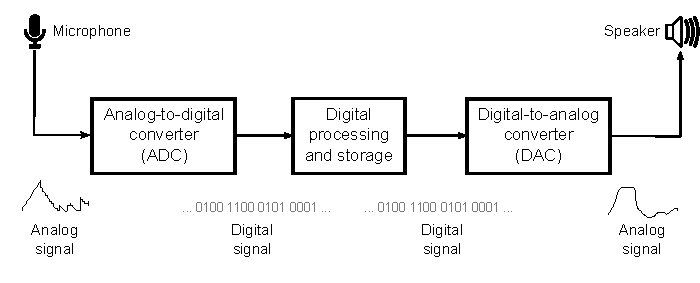
\includegraphics[height=.34\textheight]{dsp}\\[3mm]
  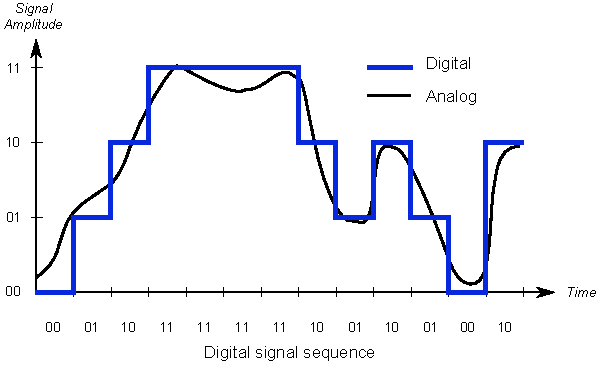
\includegraphics[height=.26\textheight]{adc}
  \begin{itemize}
    \item ADC converts the analog signal; all processing is then digital; a DAC restores analog before amplification.
    \item Sampling is periodic; each sample maps to the nearest code (here 00, 01, 10, 11).
  \end{itemize}
\end{frame}

%===============================================================================
\section{Digital Signals}
%===============================================================================

\begin{frame}{Logic Levels Are Voltage Ranges}
  \begin{columns}[c]
  \begin{column}{.5\textwidth}
    {\small\striped
    \begin{tabular}{@{}cl@{}}
      \toprule
      \textbf{Notation} & \textbf{Definition} \\
      \midrule
      $V_\mathrm{DD}$ or $V_\mathrm{CC}$ & Supply voltage \\
      $V_\mathrm{Hmin}$ & Minimum voltage for HIGH \\
      $V_\mathrm{Lmax}$ & Maximum voltage for LOW \\
      0\,V & Ground \\
      \bottomrule
    \end{tabular}}
    \vspace{3mm}
    \begin{itemize}\small
      \item Between the two ranges is \alert{undefined}; avoid it in steady state.
    \end{itemize}
  \end{column}
  \begin{column}{.48\textwidth}
    \centering
    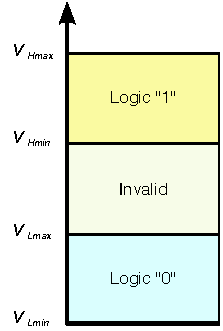
\includegraphics[height=.62\textheight]{digitalvoltages}
  \end{column}
  \end{columns}
\end{frame}

\begin{frame}{TTL, CMOS and Supply Voltage}
  \begin{itemize}
    \item \alert{TTL}: older, 5\,V supply ($V_\mathrm{CC}$).
    \item \alert{CMOS}: almost all modern logic, supply $V_\mathrm{DD}$.
    \item CMOS supplies keep falling: 3.3, 2.5, 1.8, 1.2, 1.05\,V and below.
    \item Reason: dynamic power scales as $CV^2 f$.
    \item Speed gains come from \alert{process scaling}, not lower voltage alone.
  \end{itemize}
  \begin{block}{Illustrative 3.3\,V CMOS convention}
    LOW: $0$ to $V_\mathrm{DD}/3$ ($\approx 1.1$\,V); HIGH: $2V_\mathrm{DD}/3$ ($\approx 2.2$\,V) to $V_\mathrm{DD}$.\\
    So 1\,V is LOW, 2\,V is undefined, 3\,V is HIGH. Real parts specify $V_\mathrm{IL}, V_\mathrm{IH}, V_\mathrm{OL}, V_\mathrm{OH}$ in the datasheet.
  \end{block}
\end{frame}

\begin{frame}{Timing Diagrams}
  \centering
  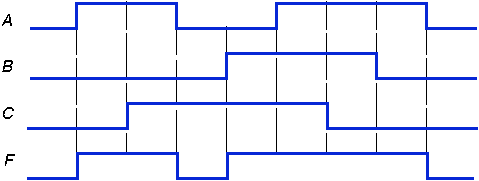
\includegraphics[height=.5\textheight]{exrajahmasa}
  \begin{itemize}
    \item A timing diagram plots logic values against \alert{time}, for one or more signals.
    \item HIGH and LOW are drawn as straight lines; transitions as vertical lines.
    \item Real transitions take time, but are short compared with the time between them.
  \end{itemize}
\end{frame}

%===============================================================================
\section{Digital Devices}
%===============================================================================

\begin{frame}{Gates and Flip-Flops}
  \begin{columns}[c]
  \begin{column}{.5\textwidth}
    \centering
    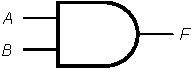
\includegraphics[height=.14\textheight]{ANSI_AND}\hspace{4mm}
    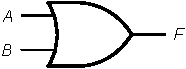
\includegraphics[height=.14\textheight]{ANSI_OR}\hspace{4mm}
    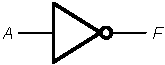
\includegraphics[height=.14\textheight]{ANSI_NOT}
    \vspace{2mm}
    \begin{itemize}\small
      \item AND: HIGH only if both inputs HIGH.
      \item OR: HIGH if at least one input HIGH.
      \item NOT: inverts its input.
      \item Output depends on present input only: \alert{combinational}.
    \end{itemize}
  \end{column}
  \begin{column}{.48\textwidth}
    \begin{block}{Flip-flops}
      Retain a 0 or 1. The stored value is the \alert{state}. Output depends on past inputs too: \alert{sequential} circuits have \emph{memory}.
    \end{block}
  \end{column}
  \end{columns}
\end{frame}

\begin{frame}{Levels of Digital Circuits}
  \begin{table}
  \centering\small\striped
  \begin{tabular}{@{}ll@{}}
    \toprule
    \textbf{Level} & \textbf{Examples} \\
    \midrule
    System    & Processors, memories \\
    Module    & Multiplexers, decoders, counters, registers \\
    Primitive & Gates, flip-flops \\
    Device    & Transistors, resistors, capacitors \\
    \bottomrule
  \end{tabular}
  \end{table}
  Lower levels are joined to build the level above.
\end{frame}

\begin{frame}{Digital Integrated Circuits}
  \begin{columns}[t]
  \begin{column}{.5\textwidth}
    {\small
    \begin{itemize}\itemsep2pt
      \item An IC puts many transistors on one silicon \alert{die}.
      \item Dies are made many to a wafer, tested, cut, then packaged.
      \item Historical classes by transistor count are only approximate.
    \end{itemize}}
  \end{column}
  \begin{column}{.5\textwidth}
    {\footnotesize\striped
    \begin{tabular}{@{}lR{.55\textwidth}@{}}
      \toprule
      \textbf{Class} & \textbf{Approx. transistors} \\
      \midrule
      SSI  & Fewer than 100 \\
      MSI  & Hundreds to thousands \\
      LSI  & Thousands to tens of thousands+ \\
      VLSI & Hundreds of thousands to millions+ \\
      ULSI & No accepted threshold \\
      \bottomrule
    \end{tabular}}
  \end{column}
  \end{columns}
  \vspace{2mm}
  A modern SoC holds tens of billions of transistors, so a design-based classification is more useful.
\end{frame}

\begin{frame}{Modern IC Types}
  \begin{table}
  \centering\footnotesize\striped
  \begin{tabular}{@{}lR{.27\textwidth}R{.2\textwidth}R{.25\textwidth}@{}}
    \toprule
    \textbf{Type} & \textbf{Function determined by} & \textbf{Flexibility} & \textbf{Typical use} \\
    \midrule
    ASIC & Fabricated design & Fixed after fabrication & Application-specific products \\
    FPGA & Configuration bitstream & Reconfigurable & Prototyping, specialized computing \\
    CPLD & Device configuration & Reconfigurable & Glue logic, small control \\
    MCU  & Firmware & Programmable & Embedded control \\
    MPU  & Software & Programmable & General-purpose computing \\
    SoC  & Hardware design and software & Depends on implementation & Phones, tablets \\
    \bottomrule
  \end{tabular}
  \end{table}
  Categories overlap: an SoC can be an ASIC; an MCU can be implemented as an ASIC.
\end{frame}

\begin{frame}{MCU, MPU and SoC}
  \begin{columns}[t]
  \begin{column}{.33\textwidth}
    \begin{block}{MPU}\small General-purpose processor; relies on external memory and peripherals.\end{block}
  \end{column}
  \begin{column}{.33\textwidth}
    \begin{block}{MCU}\small Core, memory and peripherals (timers, communication, ADC) on one chip.\end{block}
  \end{column}
  \begin{column}{.33\textwidth}
    \begin{block}{SoC}\small Most of a computing system on a chip: cores, memory controllers, GPU, accelerators.\end{block}
  \end{column}
  \end{columns}
  \vspace{3mm}
  Modern designs are described in an HDL (Verilog or VHDL) and handled by EDA tools---see Chapter~16.
\end{frame}

\begin{frame}{Packaging}
  \begin{columns}[c]
  \begin{column}{.5\textwidth}
    \centering
    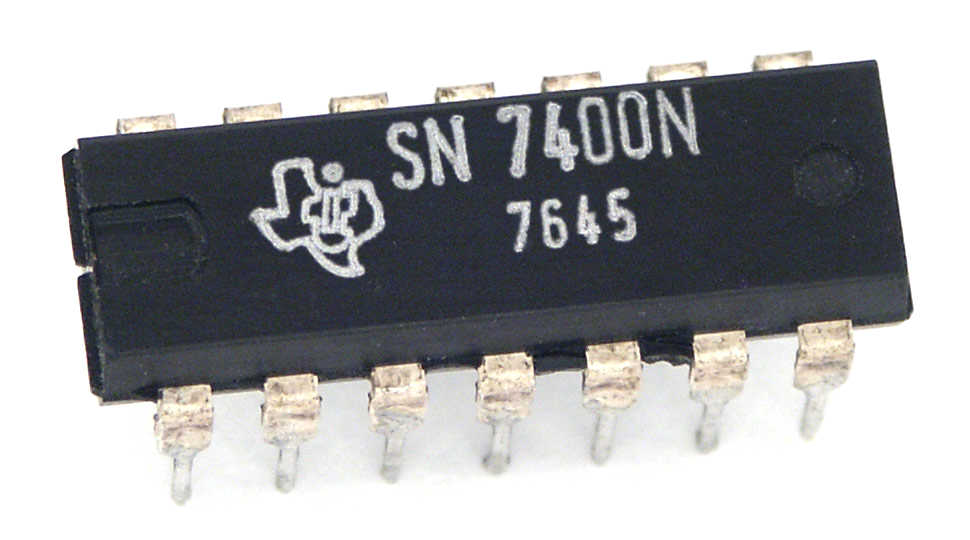
\includegraphics[height=.28\textheight]{sn7400n}\hspace{2mm}
    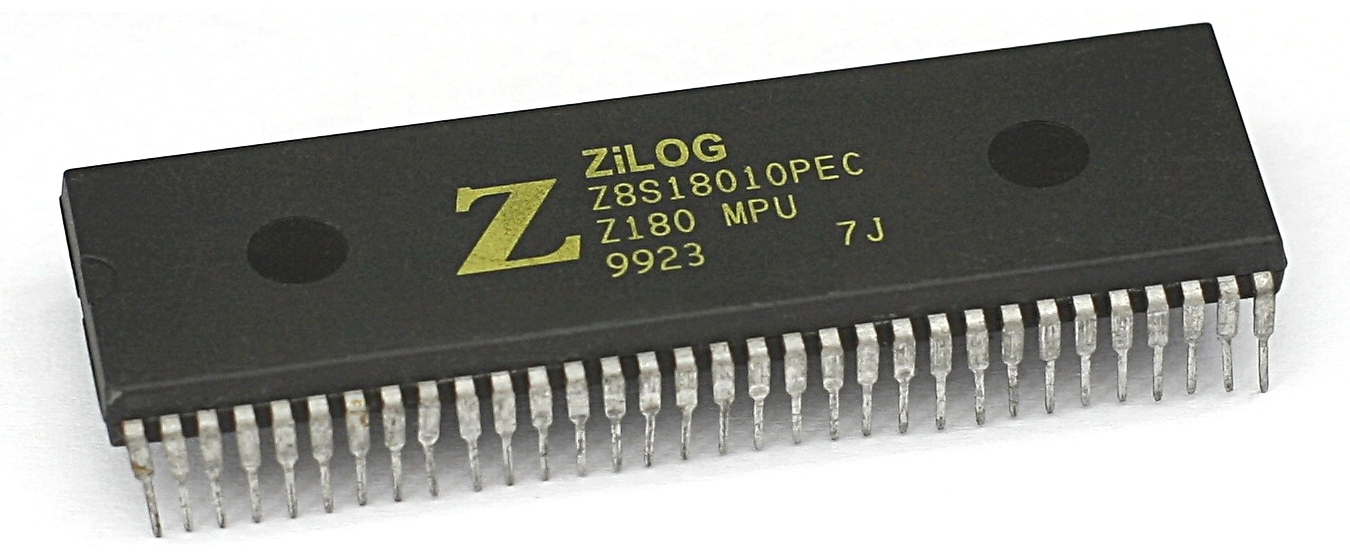
\includegraphics[height=.28\textheight]{z80dip}\\
    {\small DIP: through-hole, 0.1 in pin pitch}
    \vspace{3mm}

    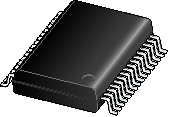
\includegraphics[height=.12\textheight]{package-soic}\hspace{2mm}
    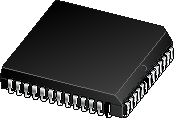
\includegraphics[height=.12\textheight]{package-plcc}\hspace{2mm}
    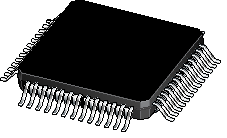
\includegraphics[height=.12\textheight]{package-qfp}\\
    {\small SMT: SOIC, PLCC, QFP}
  \end{column}
  \begin{column}{.48\textwidth}
    \begin{itemize}\small\itemsep2pt
      \item Packages protect the die and expose pins.
      \item \alert{DIP}: breadboard-friendly, but bulky.
      \item \alert{SMT} packages dominate: smaller, suited to automated assembly.
      \item Written DIP\textit{n}; $n$ is the pin count.
    \end{itemize}
  \end{column}
  \end{columns}
\end{frame}

\begin{frame}{Packages: Then and Now}
  \centering
  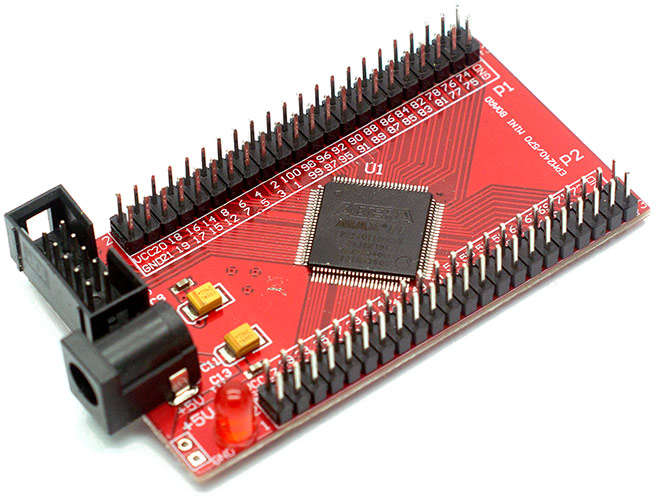
\includegraphics[height=.3\textheight]{epm240_um.jpg}\hspace{4mm}
  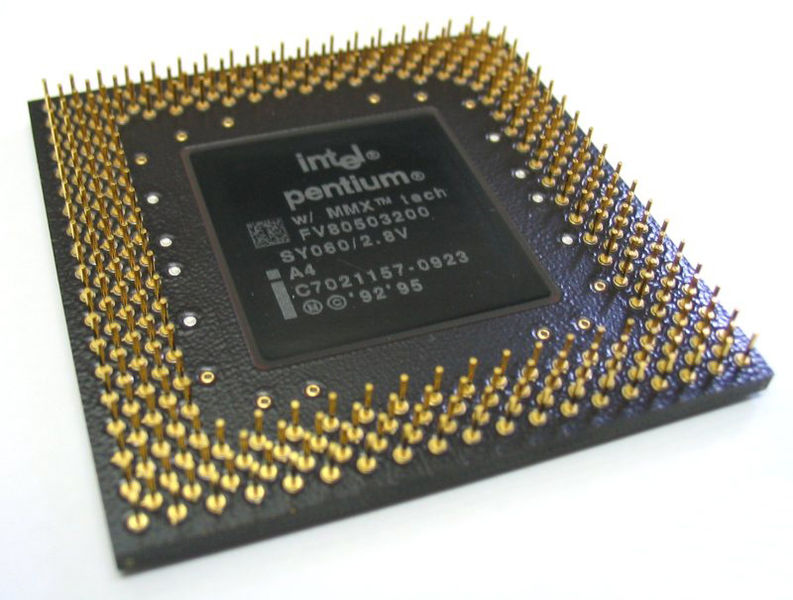
\includegraphics[height=.3\textheight]{intel-pentium}\hspace{4mm}
  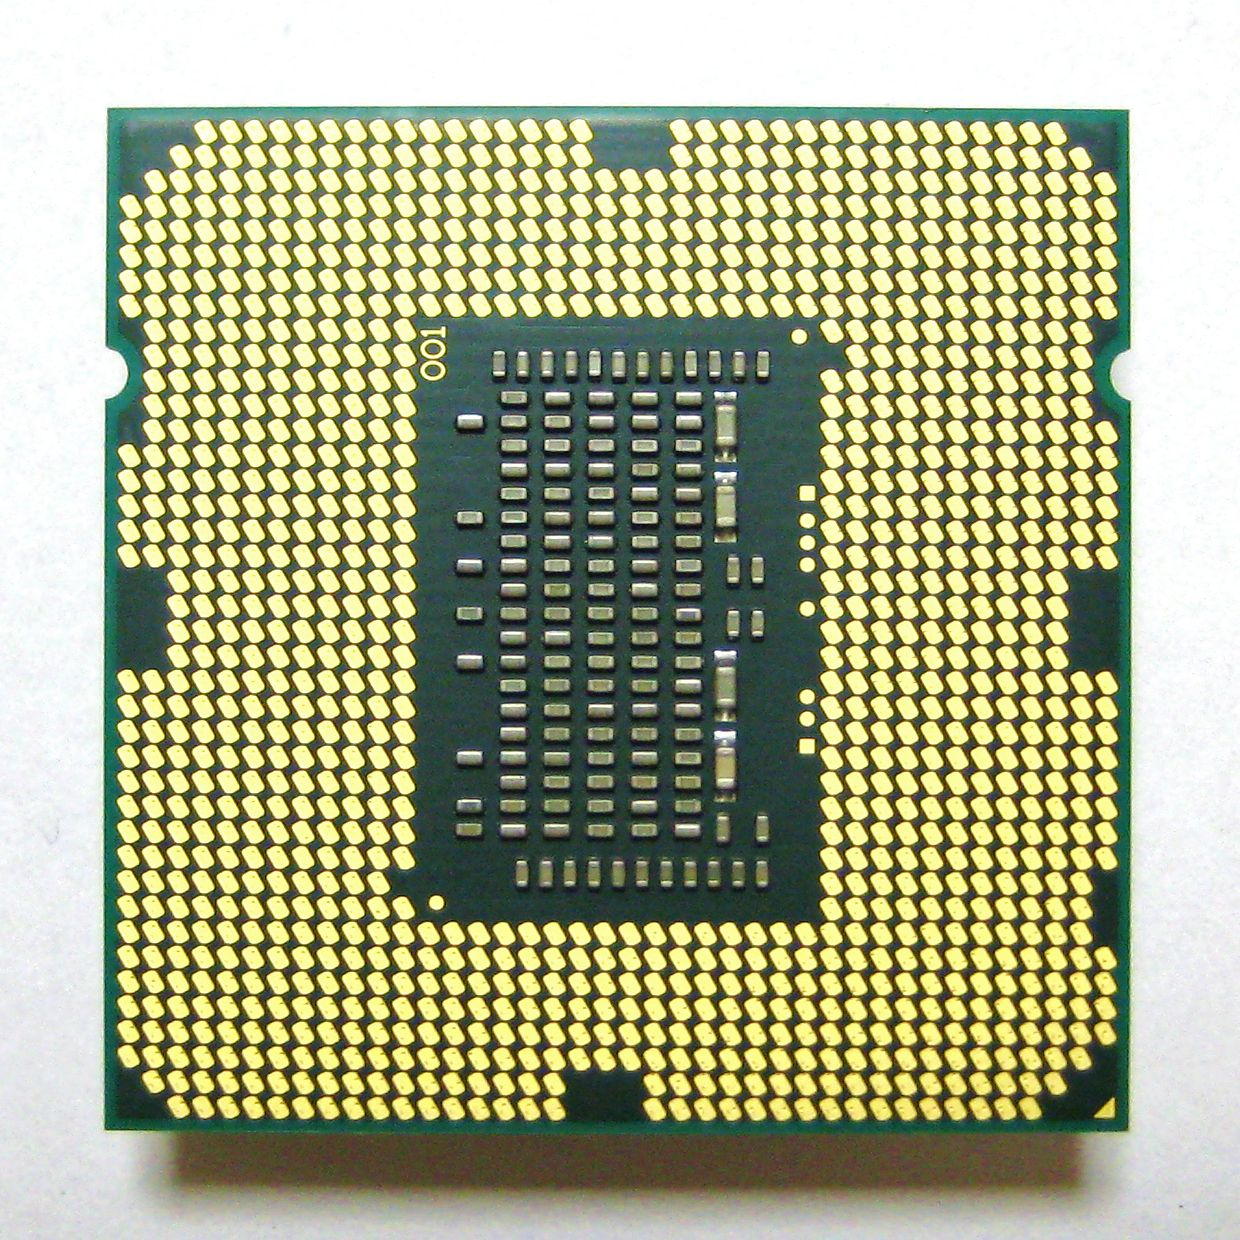
\includegraphics[height=.3\textheight]{intel-core-i5}\\[2mm]
  {\small MAX II CPLD \quad|\quad Pentium (1996): 4.5 million transistors \quad|\quad i5-750 (2009): 774 million}
\end{frame}

%===============================================================================
\section{Summary}
%===============================================================================

\begin{frame}{Summary}
  \begin{itemize}\itemsep3pt
    \item A digital signal carries one of two logic values; each is a voltage \alert{range}.
    \item ``Repeatable'', ``noise-tolerant'' and ``cheaper'' hold only under stated conditions.
    \item CMOS has displaced TTL; lower $V_\mathrm{DD}$ cuts dynamic power ($\propto CV^2 f$).
    \item Gates are combinational; flip-flops are sequential. Modules compose primitives; systems compose modules.
    \item Classify modern ICs as ASIC, FPGA, CPLD, MCU, MPU or SoC.
  \end{itemize}
  \begin{block}{Looking ahead}
    Chapter 2 shows how patterns of bits represent integers, fractions, characters and sequences.
  \end{block}
\end{frame}

\end{document}
